Detection was consistent across faults (10--15\,s to the alert, about 5\,s more until the agent was
paged and engaged), because it depends on the burn-rate windows rather than on the fault. Recovery
depended on the fix: about 21--22\,s for Redis faults healed by \act{cache\_bypass}, 35--36\,s for
crashed services that needed a restart (including the operator's 5\,s approval for
\act{restart\_postgres}). The slow database took longest (median 81.9\,s): pool timeouts made it look
unreachable, so the agent sometimes restarted PostgreSQL (with approval) before warming the cache,
the same ambiguity the bandit showed in experiments. All three compound faults were escalated after
the action budget was spent, and each escalation closed automatically once the lab was reset.

\begin{figure}[t]
\centering
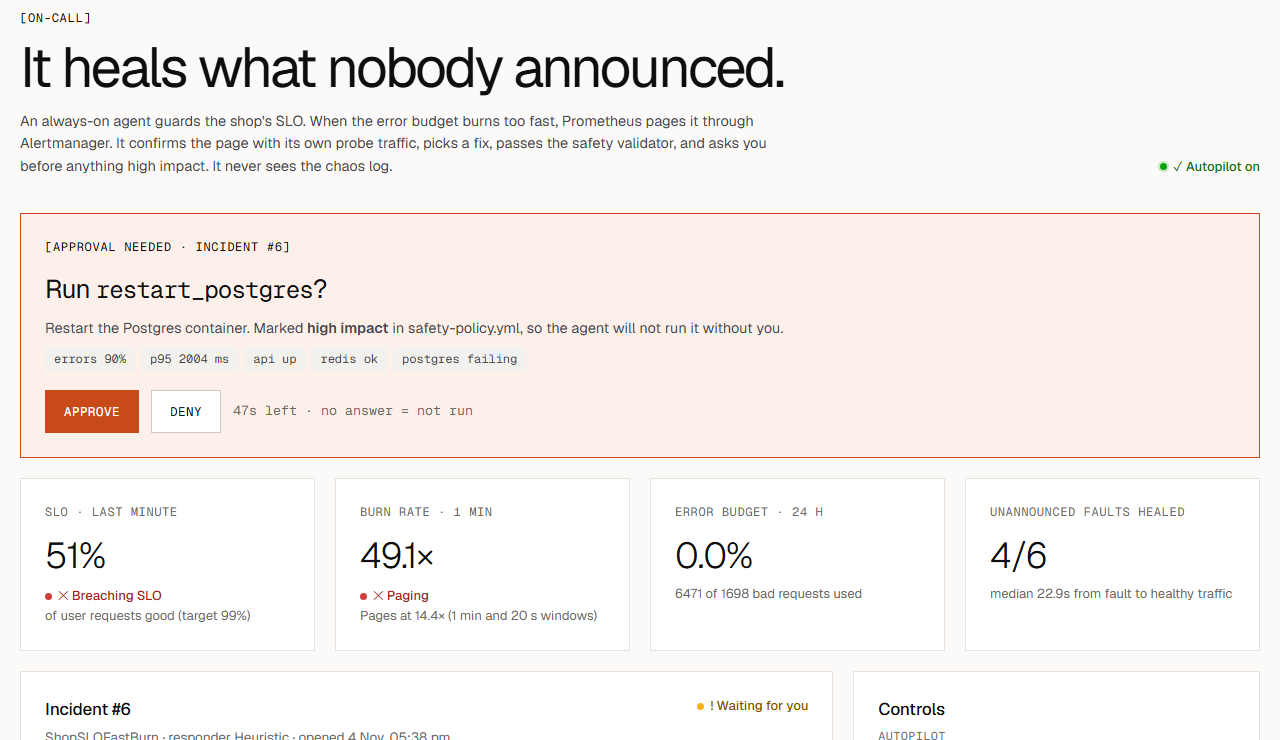
\includegraphics[width=\columnwidth]{screens/oncall-approval-crop.png}
\caption{The dashboard's on-call console during an unannounced \act{postgres\_down}: the agent proposes
the high-impact \act{restart\_postgres} and waits for a human decision; with no decision in 60\,s the
action is not run.}
\label{fig:approval}
\end{figure}
